\ylDisplay{Skeem} % Ülesande nimi
{Tundmatu autor} % Autor
{lõppvoor} % Voor
{2013} % Aasta
{P 2} % Ülesande nr.
{2} % Raskustase
{
% Teema: Elektriõpetus

\ifStatement
Leidke joonisel toodud mõõteriistade näidud. Vooluallika pinge on $U$, kõikide takistite takistused on $R$ ning mõõteriistad on ideaalsed.
\begin{center}
	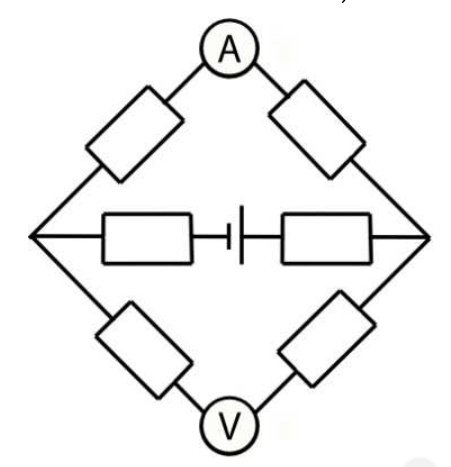
\includegraphics[width=0.5\linewidth]{2013-v3p-02-yl.png}
\end{center}
\fi

\ifHint
Ülesande lahendamisel aitab, kui skeem joonistada ümber lihtsamate jada- ja rööpühendustest koosneva segaühendusena.
\fi

\ifSolution
\begin{center}
	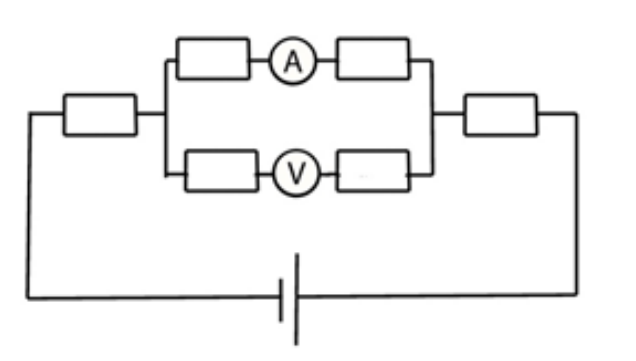
\includegraphics[width=0.5\linewidth]{2013-v3p-02-lah.png}
\end{center}
Kujutades skeemi teisiti on näha, et voltmeetriga jadamisi olevad takistid ei mõjuta tulemust, seega vooluringi kogutakistus on $4R$. Ampermeetri näit on seega $I = \frac{U}{4R}$. Voltmeeter mõõdab pinget kahel takistil kokku, seega voltmeetri näit on $U = \frac{U}{4R} 2R = U / 2$.
\fi
}